
\documentclass[12pt,notitlepage]{article}
\usepackage[utf8]{inputenc}
\usepackage{geometry}
\geometry{verbose,tmargin=1.25in,bmargin=1.25in,lmargin=1in,rmargin=1in}
\usepackage{verbatim}
\usepackage{float}
\usepackage{bm}
\usepackage{amsmath}
\usepackage{amssymb}
\usepackage{graphicx}
\usepackage{setspace}
\usepackage[authoryear]{natbib}
\usepackage{booktabs}

\onehalfspacing

\makeatletter

\usepackage{amsfonts}
\usepackage{multicol}
\usepackage{pdflscape}

\setcounter{MaxMatrixCols}{10}

\usepackage{fancyhdr}
\usepackage[utf8]{inputenc}

% This gives Roman section numbers
%\renewcommand{\thesection}{\Roman{section}} 
%\renewcommand{\thesubsection}{\thesection.\Alph{subsection}}

% This gives assumption numbers
\usepackage{amsmath}  
%\newtheorem{assumption}{Assumption}
%\newtheorem{lemma}{Lemma}

% Scalars
%\input{../input/results/scalars}

%\usepackage[latin9]{inputenc}
%\usepackage{geometry}
%\geometry{verbose,tmargin=1in,bmargin=1in,lmargin=1in,rmargin=1in}
\usepackage{float}
\usepackage{amsthm}
\usepackage{amsmath}
\usepackage{amssymb}
\usepackage{graphicx}
\usepackage{setspace}
\doublespace
\usepackage{esint}  
\usepackage[authoryear]{natbib}
\usepackage{hyperref}
\usepackage{comment}
\usepackage[normalem]{ulem}
\usepackage{array}
\usepackage{multirow}
\usepackage{float}
\usepackage{cancel}
\usepackage{enumerate}
\makeatletter
\makeatother
%\numberwithin{equation}{section} %numbering equation with section number
\usepackage{pgf,tikz}
\usepackage{mathrsfs}
\usetikzlibrary{arrows}
\usepackage[english]{babel}


\theoremstyle{plain}
\newtheorem{theorem}{\protect\theoremname}
\theoremstyle{plain}
\newtheorem*{theorem*}{\protect\theoremname}
\theoremstyle{definition}
\newtheorem{definition}{\protect\definitionname}
\theoremstyle{definition}
\newtheorem*{definition*}{\protect\definitionname}
\theoremstyle{assumption}
\newtheorem{assumption}{\protect\assumptionname}
\theoremstyle{plain}
\newtheorem{corollary}{\protect\corollaryname}
\theoremstyle{plain}
\newtheorem{lemma}{\protect\lemmaname}
\theoremstyle{plain}
\newtheorem{proposition}{\protect\propositionname}
\theoremstyle{plain}
\newtheorem{conjecture}{\protect\conjecturename}
\theoremstyle{definition}%%%12/28/2019
\newtheorem{remark}{\protect\remarkname}
\theoremstyle{plain}
\newtheorem{claim}{\protect\claimname}
\theoremstyle{plain}
\newtheorem{fact}{\protect\factname}
\theoremstyle{plain}
\newtheorem{result}{\protect\resultname}
\theoremstyle{plain}
\newtheorem{observation}{\protect\observationname}

\providecommand{\claimname}{Claim}
\providecommand{\conjecturename}{Conjecture}
\providecommand{\corollaryname}{Corollary}
\providecommand{\lemmaname}{Lemma}
\providecommand{\definitionname}{Definition}
\providecommand{\assumptionname}{Assumption}
\providecommand{\examplename}{Example}
\providecommand{\factname}{Fact}
\providecommand{\propositionname}{Proposition}
\providecommand{\remarkname}{Remark}
\providecommand{\theoremname}{Theorem}
\providecommand{\resultname}{Result}
\providecommand{\observationname}{Observation}


\usepackage{subcaption}
\makeatletter
\renewcommand{\fnum@figure}{Figure \thefigure}
\makeatother

%%%%%%%%%%OWN%%%%%%%%%%%%%%%%%%%%%%%%%%%%%%%%%%%%%%%%%%%%%%%%%%%%%%%%%%%%%%%%%%%%%%%%%%%%%%%%%%%%%%%%%%%%%%%%%%%%%%%%%%%%%%%
\usepackage[font=footnotesize]{caption} 

\usepackage{physics}
\usepackage{enumitem}
\usepackage{pgfplots}
\usepackage{mathtools}
\newcommand*\diff{\mathop{}\!\mathrm{d}}

\DeclareMathOperator*{\argmax}{arg\,max}
\DeclareMathOperator*{\argmin}{arg\,min}
\DeclareMathOperator{\supp}{Supp}
\DeclareMathOperator{\proj}{Proj}
\DeclareMathOperator{\prob}{Pr}


\usepackage{istgame}
\usetikzlibrary{shapes.geometric,arrows}

\usepackage{xcolor}
\usepackage{wrapfig}

\newcommand{\pdfcolor}{blue!85!black}
\hypersetup{colorlinks=true,linkcolor=\pdfcolor,citecolor=\pdfcolor,urlcolor=\pdfcolor}


\usepackage{bm}

\makeatother

\begin{document}

Additional pre-specified heterogeneity:

\begin{figure}[H]
\caption{Heterogeneity by Willingness to Donate to a Climate-Related Cause \label{fig:hte_donation}}
\medskip{}
\begin{centering}
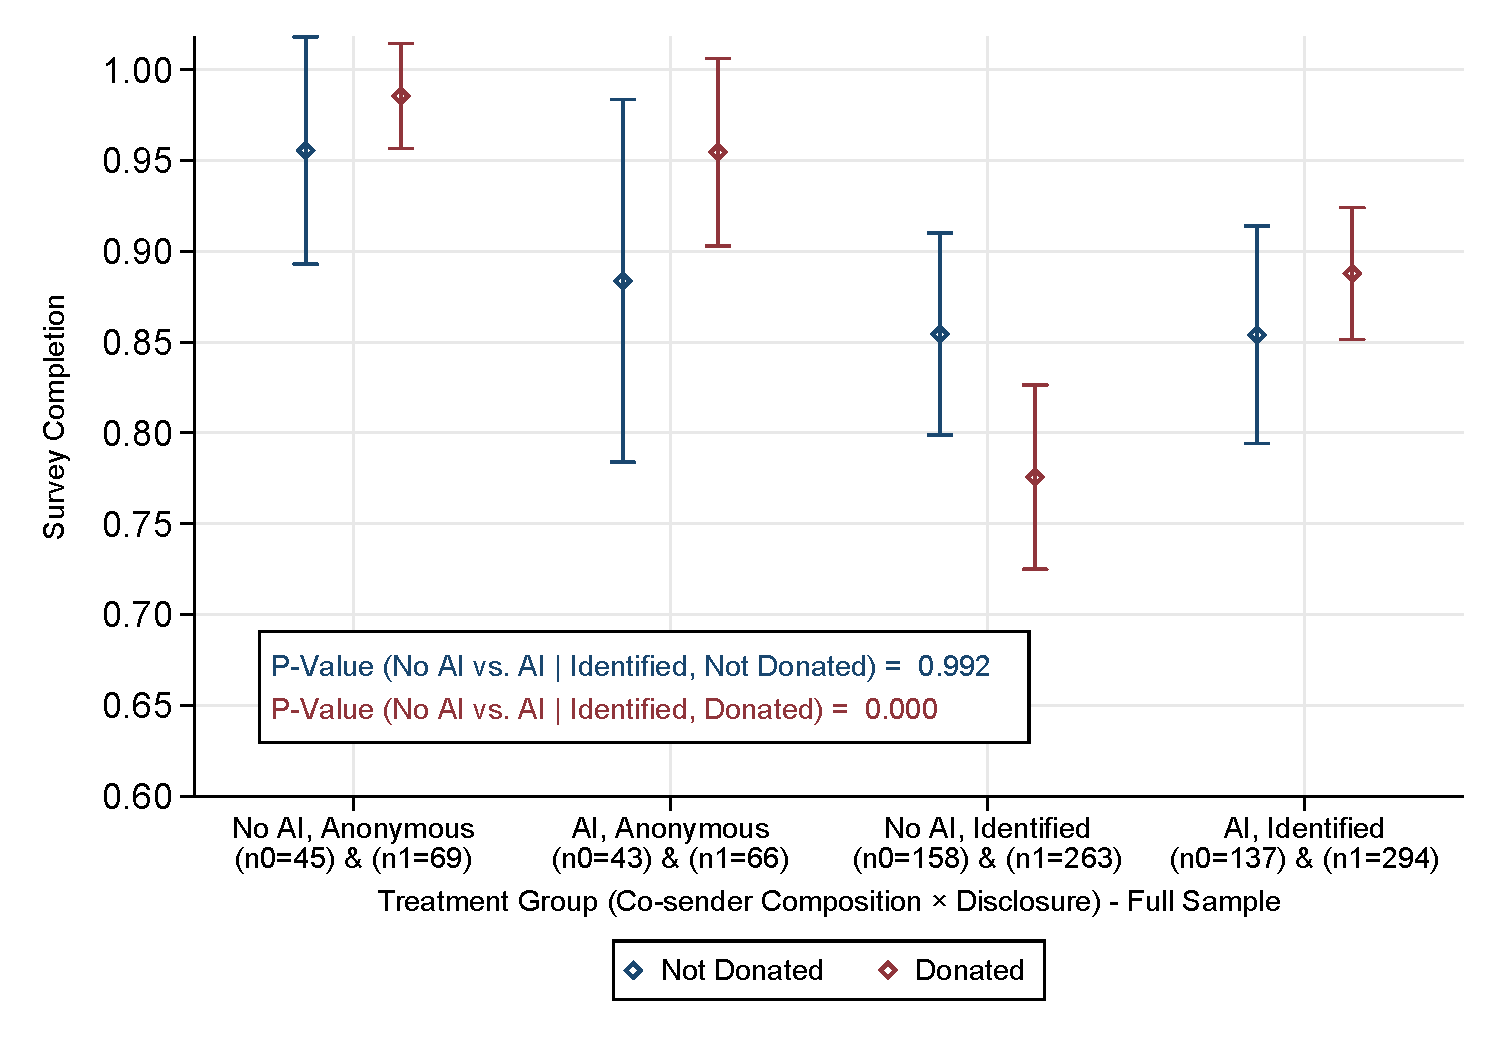
\includegraphics[width=0.9\textwidth]{figures/ciplot_Finished_hte_DonationBinary_pos_Full_raw.pdf}
\par\end{centering}
{\small{}Notes: This figure reports treatment effects on study completion by willingness to donate to a climate-related cause, used as a measure of prosociality. Respondents are classified as willing or unwilling to donate. Estimates are based on respondents who passed the attention check. Error bars denote 95\% confidence intervals.}{\small\par}
\end{figure}

\begin{figure}[H]
\caption{Heterogeneity by Baseline Attitudes Toward Climate Change \label{fig:hte_climate}}
\medskip{}
\begin{centering}
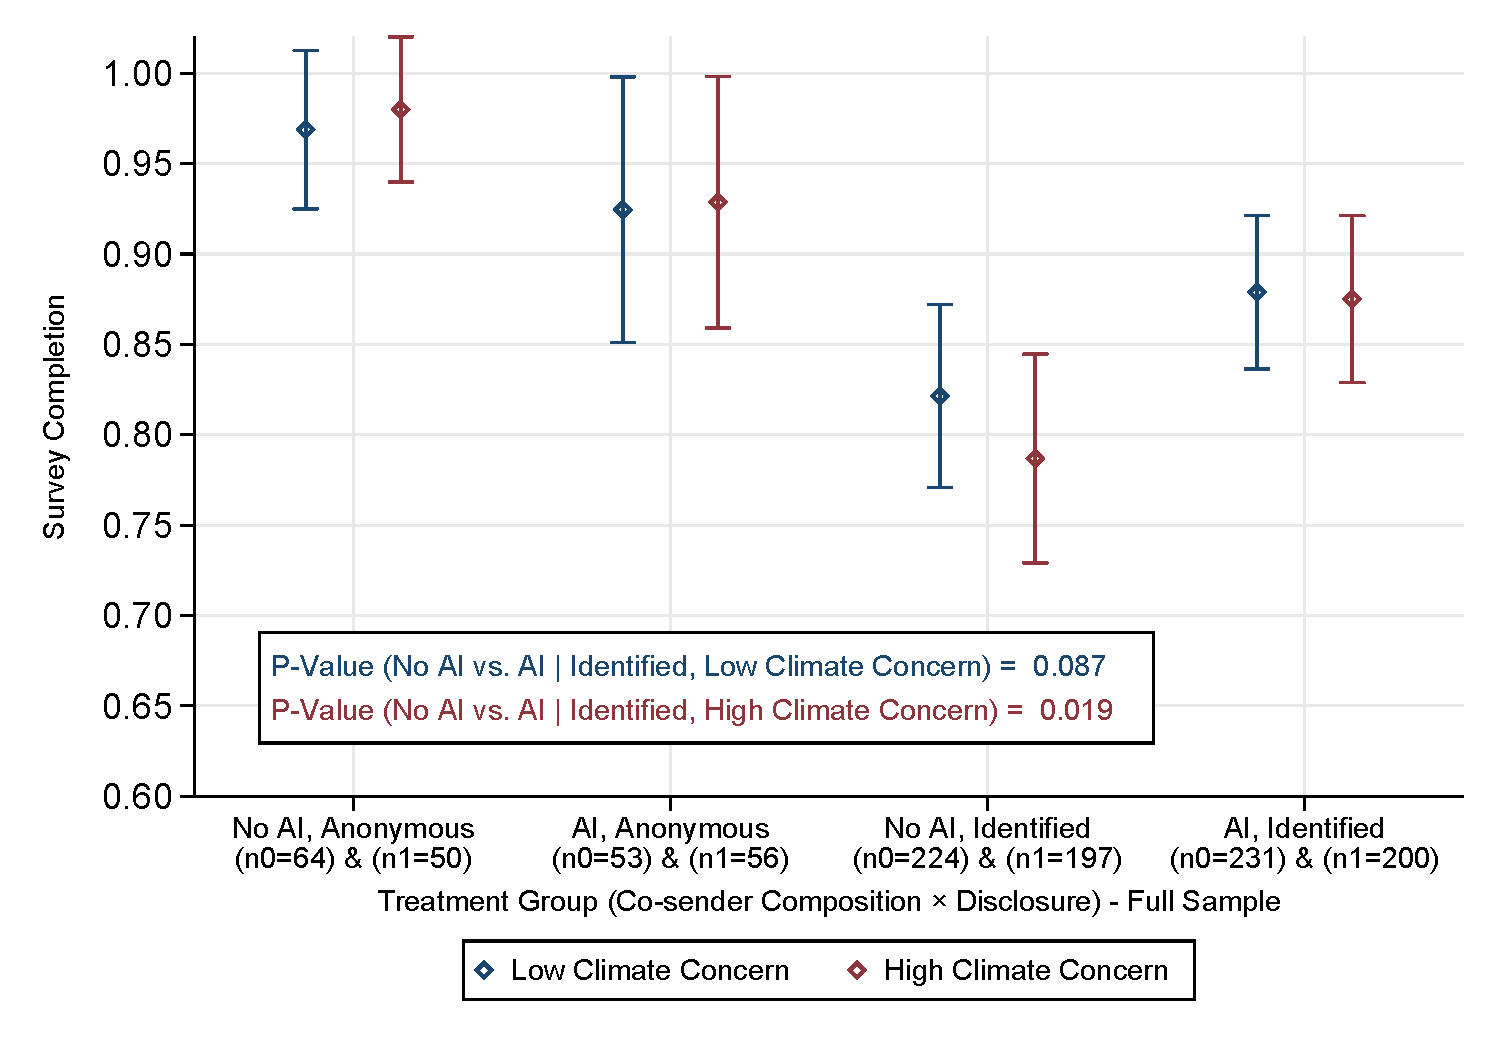
\includegraphics[width=0.9\textwidth]{figures/ciplot_Finished_hte_index_ClimateBinary_Full_raw.pdf}
\par\end{centering}
{\small{}Notes: This figure reports treatment effects on study completion by baseline attitudes toward climate change. Attitudes are defined relative to the sample median, with respondents classified as below-median or above-median. Estimates are based on respondents who passed the attention check. Error bars denote 95\% confidence intervals.}{\small\par}
\end{figure}

\begin{figure}[H]
\caption{Heterogeneity by Image Concerns \label{fig:hte_image}}
\medskip{}
\begin{centering}
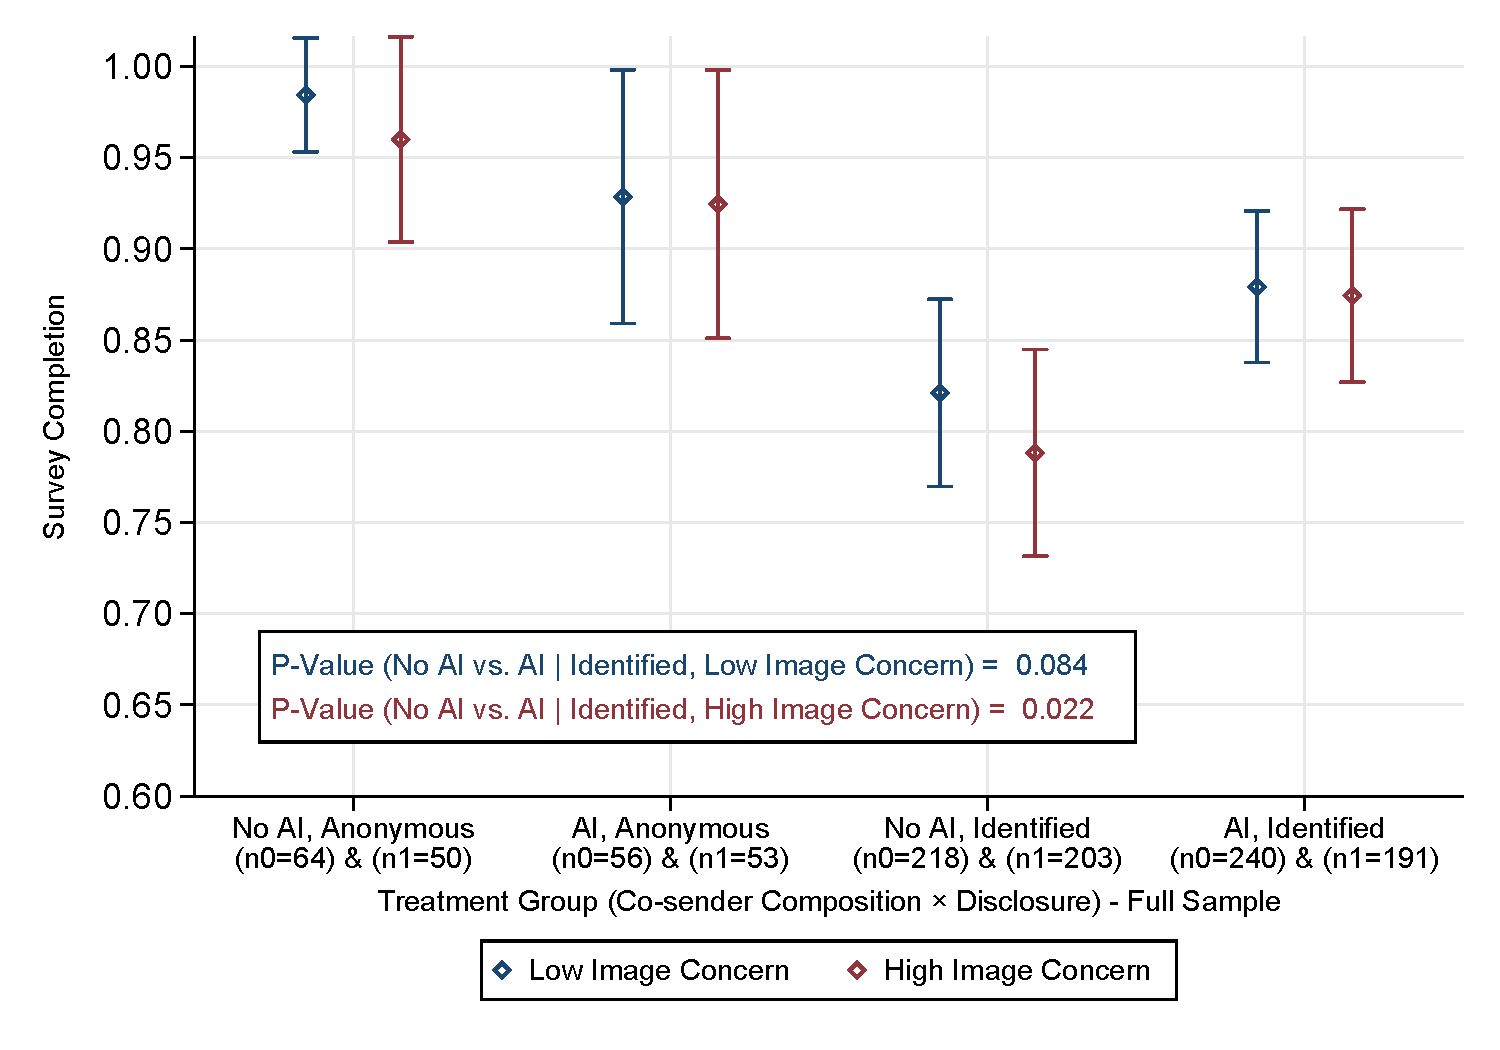
\includegraphics[width=0.9\textwidth]{figures/ciplot_Finished_hte_ImageConcernBinary_p50_Full_raw.pdf}
\par\end{centering}
{\small{}Notes: This figure reports treatment effects on study completion by image concerns. Image concerns are defined relative to the sample median, with respondents classified as below-median or above-median. Estimates are based on respondents who passed the attention check. Error bars denote 95\% confidence intervals.}{\small\par}
\end{figure}


\begin{figure}[H]
\caption{Heterogeneity by Baseline Perceived Difference Between Own Writing and AI-Generated Content \label{fig:hte_aidiff}}
\medskip{}
\begin{centering}
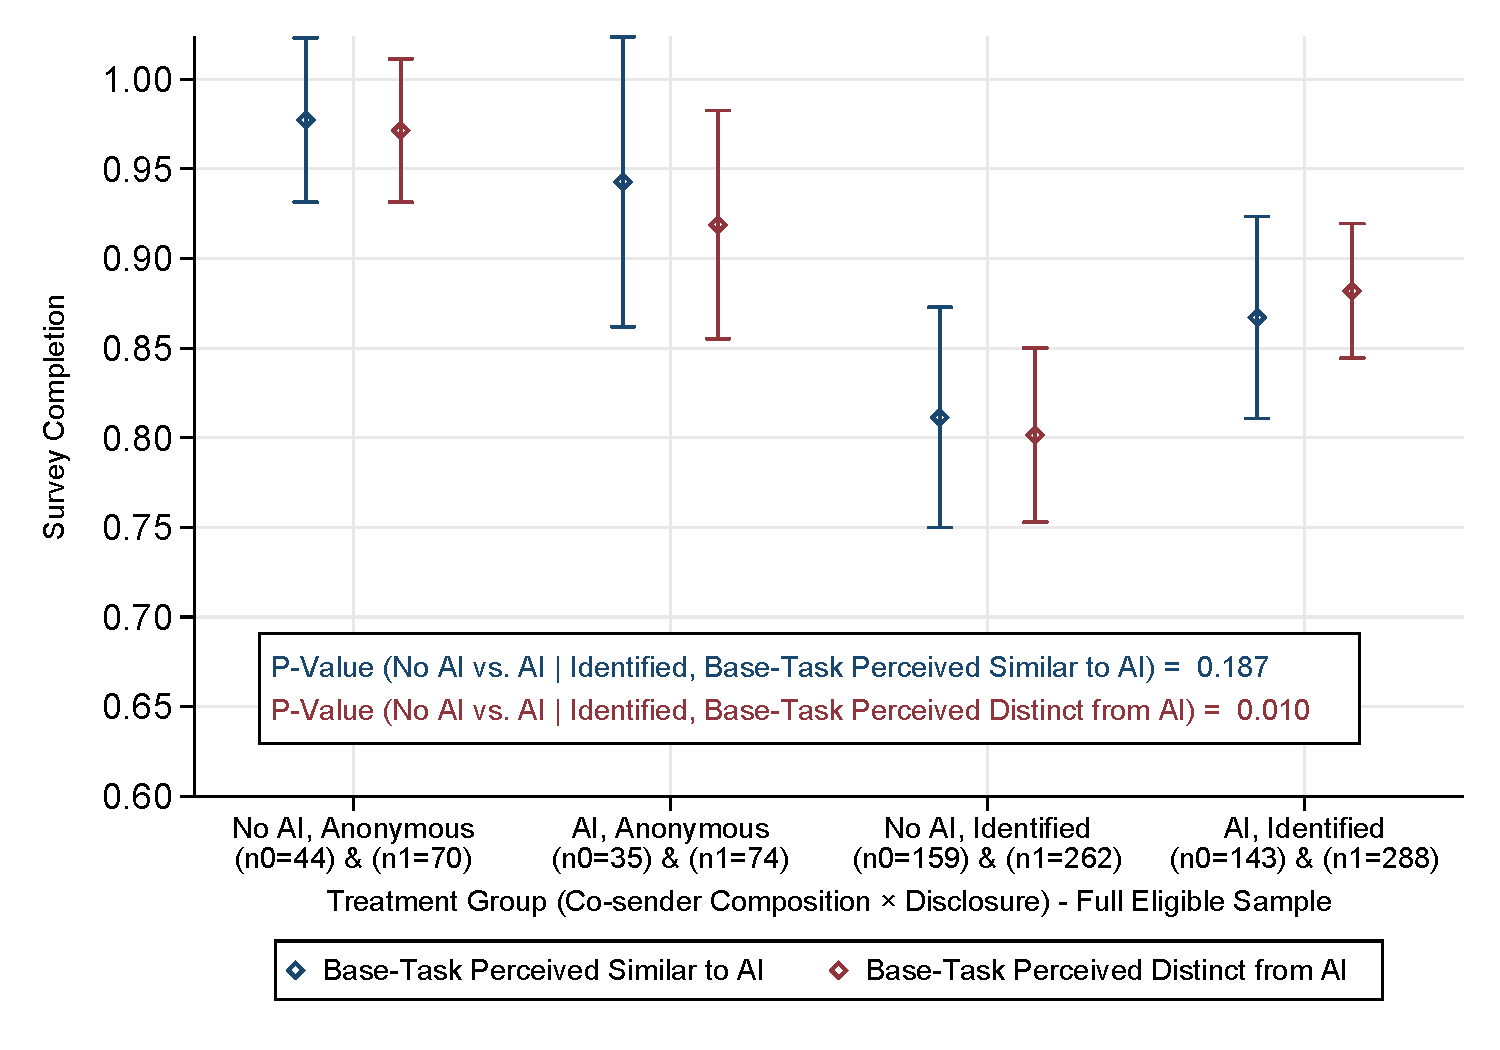
\includegraphics[width=0.9\textwidth]{figures/ciplot_Finished_hte_AIDiffBinary_Full_raw.pdf}
\par\end{centering}
{\small{}Notes: This figure reports treatment effects on study completion by baseline perceived difference between one's own writing and AI-generated content. Perceived difference is defined relative to the sample median, with respondents classified as below-median or above-median. Estimates are based on respondents who passed the attention check. Error bars denote 95\% confidence intervals.}{\small\par}
\end{figure}



Additional pre-specified figures collected after the writing task (for completed / post attrition sample):


Secondary outcomes:
\begin{figure}[H]
\caption{Perceived Effectiveness of AI \label{fig:genai_effective}}
\medskip{}
\begin{centering}
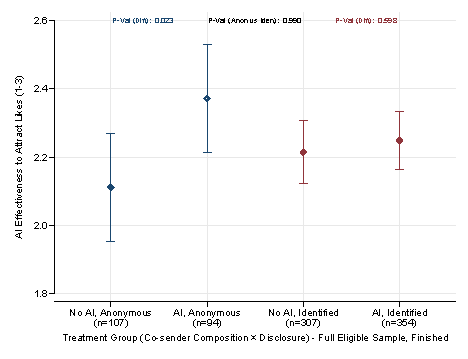
\includegraphics[width=0.9\textwidth]{figures/ciplot_GenAIEffective_Full_raw_finished.pdf}
\par\end{centering}
{\small{}Notes: This figure reports treatment effects on perceived effectiveness of AI. Estimates are based on respondents who passed the attention check and completed the survey. Error bars denote 95\% confidence intervals.}{\small\par}
\end{figure}


\begin{figure}[H]
\caption{Perceived AI-ness of Own Writing \label{fig:perceive_ai}}
\medskip{}
\begin{centering}
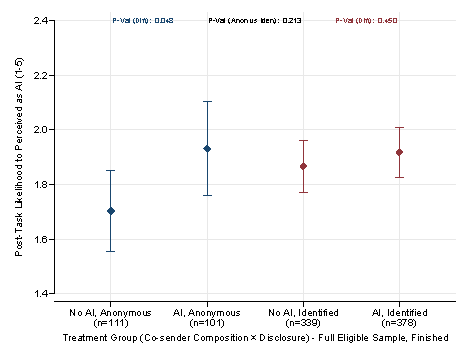
\includegraphics[width=0.9\textwidth]{figures/ciplot_PerceiveAI_Full_raw_finished.pdf}
\par\end{centering}
{\small{}Notes: This figure reports treatment effects on the perceived AI-ness of own writing. Respondents were asked how likely they believe their audience would identify their post as AI-generated. Estimates are based on respondents who passed the attention check and completed the survey. Error bars denote 95\% confidence intervals.}{\small\par}
\end{figure}


\begin{figure}[H]
\caption{Importance of Being Perceived Positively by Others \label{fig:signal_value}}
\medskip{}
\begin{centering}
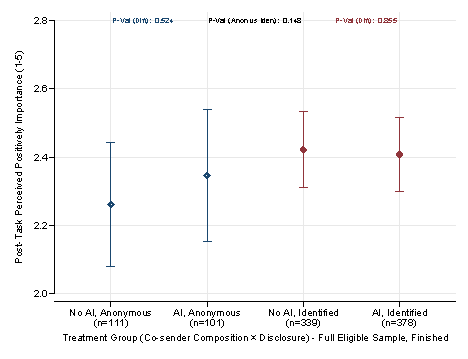
\includegraphics[width=0.9\textwidth]{figures/ciplot_SignalValue_Full_raw_finished.pdf}
\par\end{centering}
{\small{}Notes: This figure reports treatment effects on the importance of being perceived positively by others. Estimates are based on respondents who passed the attention check and completed the survey. Error bars denote 95\% confidence intervals.}{\small\par}
\end{figure}


\begin{figure}[H]
\caption{Perceived Engagement on Climate Change \label{fig:perceive_engaged}}
\medskip{}
\begin{centering}
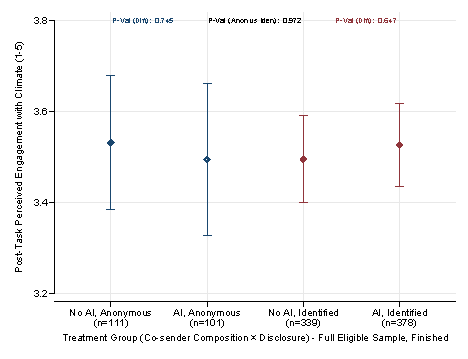
\includegraphics[width=0.9\textwidth]{figures/ciplot_PerceiveEngaged_Full_raw_finished.pdf}
\par\end{centering}
{\small{}Notes: This figure reports treatment effects on perceived engagement on climate change issues. Respondents were asked how engaged they think they will seem to their audience on issues of climate change. Estimates are based on respondents who passed the attention check and completed the survey. Error bars denote 95\% confidence intervals.}{\small\par}
\end{figure}


\begin{figure}[H]
\caption{Post AI-ness \label{fig:post_ainess}}
\medskip{}
\begin{centering}
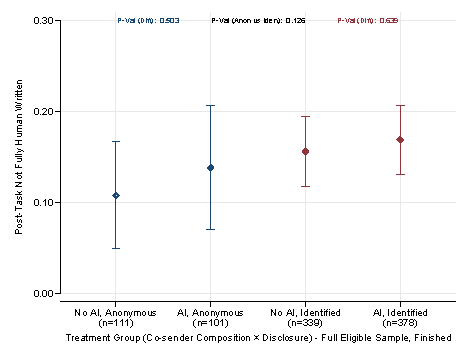
\includegraphics[width=0.9\textwidth]{figures/ciplot_Post_AIness_Full_raw_finished.pdf}
\par\end{centering}
{\small{}Notes: This figure reports treatment effects on post AI-ness as measured by Pangram AI detection. Estimates are based on respondents who passed the attention check and completed the survey. Error bars denote 95\% confidence intervals.}{\small\par}
\end{figure}

\begin{figure}[H]
\caption{Post Content Index: Textual Features \label{fig:post_effort}}
\medskip{}
\begin{centering}
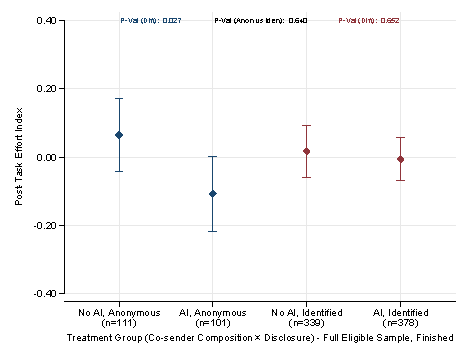
\includegraphics[width=0.9\textwidth]{figures/ciplot_index_Post_effort_Full_raw_finished.pdf}
\par\end{centering}
{\small{}Notes: This figure reports treatment effects on an index of post effort, comprising text length, average sentence length, and typo rate (normalized by text length, sign-reversed). Estimates are based on respondents who passed the attention check and completed the survey. Error bars denote 95\% confidence intervals.}{\small\par}
\end{figure}

\begin{figure}[H]
\caption{Post Content Index: Rhetorical Features \label{fig:post_nlp}}
\medskip{}
\begin{centering}
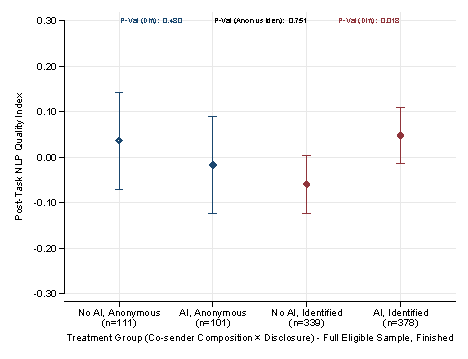
\includegraphics[width=0.9\textwidth]{figures/ciplot_index_Post_nlp_Full_raw_finished.pdf}
\par\end{centering}
{\small{}Notes: This figure reports treatment effects on an index of post content, comprising NLP-based measures of the use of personal anecdotes, emotional appeals, scientific arguments, and causal narratives. Estimates are based on respondents who passed the attention check and completed the survey. Error bars denote 95\% confidence intervals.}{\small\par}
\end{figure}

\end{document}